\documentclass[a4paper,11pt]{article}
\usepackage[margin=2.35cm,top=1.25cm,bottom=1.55cm,headheight=16pt,headsep=8pt,footskip=22pt]{geometry}
\usepackage[T1]{fontenc}
\usepackage[utf8]{inputenc}
\usepackage{lmodern}
\usepackage{graphicx}
\usepackage{xcolor}
\usepackage{array}
\usepackage{tabularx}
\usepackage{booktabs}
\usepackage{enumitem}
\usepackage{tikz}
\usepackage{tcolorbox}
\tcbuselibrary{skins,breakable}
\usepackage{fancyhdr}
\usepackage{needspace}
\usepackage{hyperref}
\usepackage{microtype}
\usetikzlibrary{positioning,arrows.meta,calc}

\definecolor{GEUBlue}{RGB}{64,102,150}
\definecolor{GEUDark}{RGB}{26,47,70}
\definecolor{BoxGrey}{RGB}{245,245,245}
\hypersetup{colorlinks=true,urlcolor=GEUBlue,linkcolor=GEUBlue}
\setlength{\parindent}{0pt}
\setlength{\parskip}{5pt}
\setlength{\tabcolsep}{5pt}
\renewcommand{\arraystretch}{1.12}

\pagestyle{fancy}
\fancyhf{}
\fancyhead[L]{\scriptsize\bfseries DSCPP-III-2026-T238}
\fancyhead[R]{\scriptsize\bfseries PROJECT PROPOSAL}
\fancyfoot[L]{\scriptsize Department of Computer Science \& Engineering - Graphic Era (Deemed to be University)}
\fancyfoot[R]{\scriptsize Page~\thepage}
\renewcommand{\headrulewidth}{0pt}
\renewcommand{\footrulewidth}{0pt}

\newcommand{\MainHeading}[1]{{\color{GEUBlue}\fontsize{20}{23}\selectfont\bfseries #1\par}\vspace{5pt}}
\newcommand{\SubHeading}[1]{\needspace{3\baselineskip}{\color{GEUBlue}\fontsize{15.5}{18}\selectfont #1\par}\vspace{1pt}}
\newcommand{\Instruction}[1]{{\itshape #1\par}\vspace{5pt}}
\newtcolorbox{answerbox}[1][]{enhanced,colback=white,colframe=black!70,boxrule=0.6pt,arc=0pt,left=8pt,right=8pt,top=7pt,bottom=7pt,breakable,#1}
\newtcolorbox{softbox}[1][]{enhanced,colback=BoxGrey,colframe=BoxGrey,boxrule=0pt,arc=1pt,left=8pt,right=8pt,top=6pt,bottom=6pt,breakable,#1}

\newcommand{\memberrow}[5]{%
\textbf{#1}\\[-1pt]
{\itshape (#2)} &
\begin{minipage}[t]{\linewidth}\small
\textit{#3}\\[3pt]
\centering\includegraphics[height=2.1cm,keepaspectratio]{#4}\end{minipage}\\
\hline
}

\begin{document}

% PAGE 1
\MainHeading{PROJECT AND TEAM INFORMATION}
\SubHeading{Project Title}
\Instruction{(Try to choose a catchy title. Max 20 words).}
\begin{answerbox}
TeamForge - Skill-Based Hackathon \& Project Team Matchmaker
\end{answerbox}
\vspace{8pt}
\SubHeading{Student / Team Information}
\renewcommand{\arraystretch}{1.0}
\begin{tabularx}{\textwidth}{|>{\raggedright\arraybackslash}p{0.65\textwidth}|>{\raggedright\arraybackslash}X|}
\hline
\begin{minipage}[t]{\linewidth}
\textit{Team Name:}\\[2pt]
\textit{Team \#:}
\end{minipage}
&
\begin{minipage}[t]{\linewidth}
\textit{TEAMFORGE}\\[2pt]
\textit{DSCPP-III-2026-T238}
\end{minipage}
\\[6pt] \hline
\begin{minipage}[t][3.05cm][t]{\linewidth}
\textbf{Team member 1 (Team Lead)}\\[-1pt]
{\itshape (Last Name, name: student ID: email, picture):}
\end{minipage}
&
\begin{minipage}[t][3.05cm][t]{\linewidth}\small
\textit{Fartiyal, Mukul - 2510370466}\\[-1pt]
\textit{mukulfartiyal77@gmail.com}\\[4pt]
\centering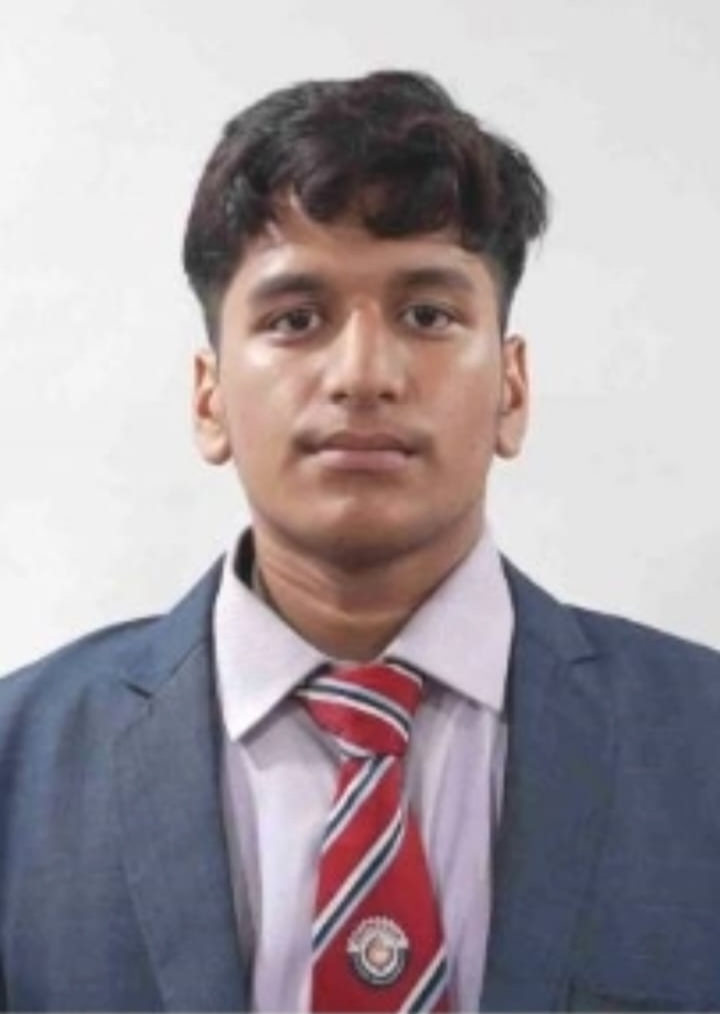
\includegraphics[height=2.15cm,keepaspectratio]{images/member1.jpeg}
\end{minipage}
\\ \hline
\begin{minipage}[t][3.05cm][t]{\linewidth}
\textbf{Team member 2}\\[-1pt]
{\itshape (Last Name, name: student ID: email, picture):}
\end{minipage}
&
\begin{minipage}[t][3.05cm][t]{\linewidth}\small
\textit{Bisht, Anubhav - 2510370178}\\[-1pt]
\textit{anubhav6875@gmail.com}\\[4pt]
\centering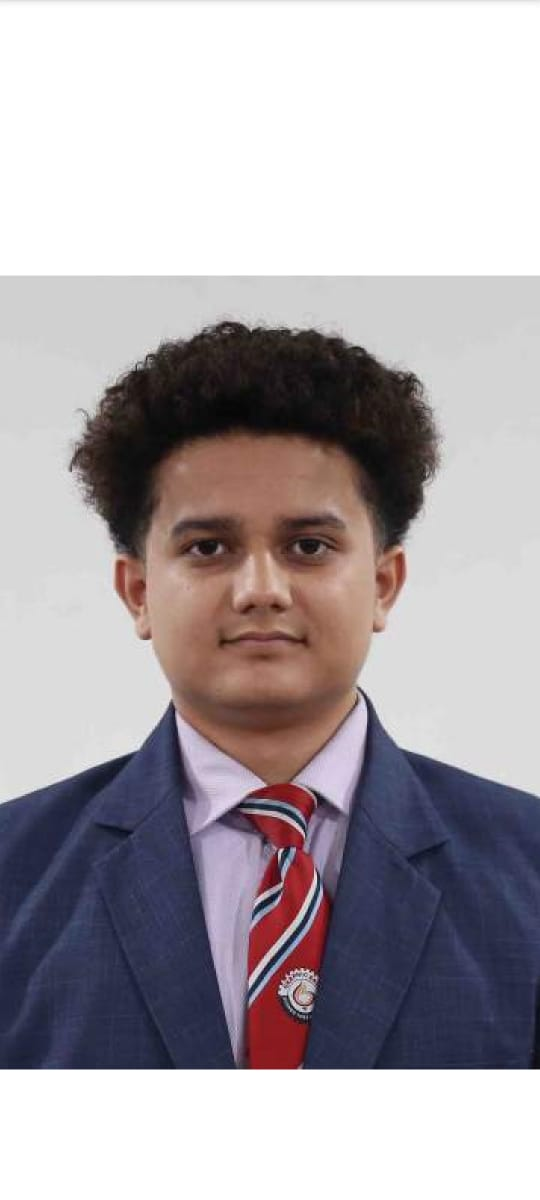
\includegraphics[height=2.15cm,keepaspectratio]{images/member2.jpeg}
\end{minipage}
\\ \hline
\begin{minipage}[t][3.05cm][t]{\linewidth}
\textbf{Team member 3}\\[-1pt]
{\itshape (Last Name, name: student ID: email, picture):}
\end{minipage}
&
\begin{minipage}[t][3.05cm][t]{\linewidth}\small
\textit{Singh, Siddhant - 2510380233}\\[-1pt]
\textit{siddhantsingh1890@gmail.com}\\[4pt]
\centering
\includegraphics[height=2.15cm,keepaspectratio]{images/member3.jpeg}
\end{minipage}
\\ \hline
\begin{minipage}[t][3.05cm][t]{\linewidth}
\textbf{Team member 4}\\[-1pt]
{\itshape (Last Name, name: student ID: email, picture):}
\end{minipage}
&
\begin{minipage}[t][3.05cm][t]{\linewidth}\small
\textit{Mehul - 2510370093}\\[-1pt]
\textit{mehul.200702@gmail.com}\\[4pt]
\centering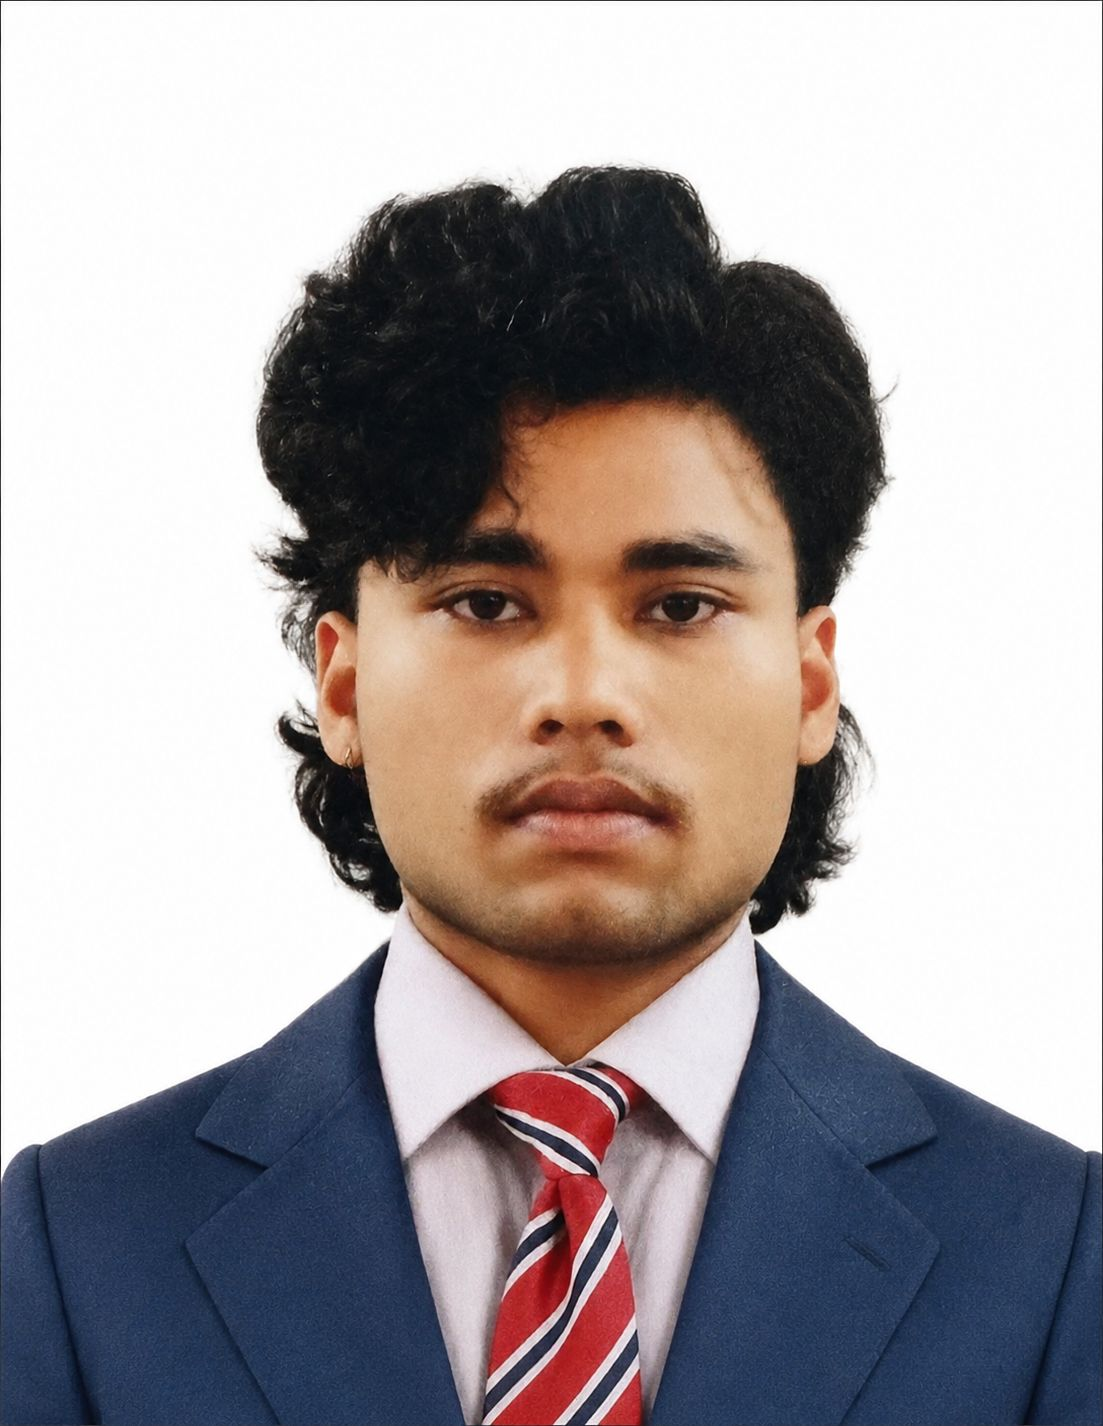
\includegraphics[height=2.15cm,keepaspectratio]{images/member4.jpeg}
\end{minipage}
\\ \hline
\end{tabularx}
\vfill
\clearpage

% PAGE 2
\MainHeading{PROPOSAL DESCRIPTION (10 pts)}
\SubHeading{Motivation (1 pt)}
\Instruction{(Describe the problem you want to solve and why it is important. Max 300 words).}
\begin{answerbox}
\begin{itemize}[leftmargin=18pt,itemsep=3pt,topsep=2pt]
\item Students usually form hackathon, PBL, or project teams through friends, existing groups, or quick messages in class groups.
\item This is convenient, but it can leave a team with several people who have similar skills while another required role is not covered.
\item Students already know useful information about themselves, such as the skills they can offer, skills they want to learn, experience level, and availability. Projects can also list the roles and skills they need.
\item TeamForge brings these two sides together. A student creates a skill profile, while a project or hackathon defines its requirements. The system then retrieves suitable candidates, calculates a compatibility score, and ranks them.
\item The team can also be checked for covered skills and remaining gaps. The final choice is still made by the students, but the comparison becomes more structured and easier to review.
\end{itemize}
\end{answerbox}
\vspace{8pt}
\SubHeading{State of the Art / Current solution (1 pt)}
\Instruction{(Describe how the problem is solved today (if it is). Max 200 words).}
\begin{answerbox}
\begin{itemize}[leftmargin=18pt,itemsep=3pt,topsep=2pt]
\item In most college settings, students use WhatsApp, Discord, class groups, friend circles, or personal contacts to find teammates.
\item Some teams compare skills manually or keep simple lists in spreadsheets. This becomes harder when the number of students and required skills increases.
\item General collaboration and profile tools can help people connect, but they do not necessarily show which available students fit a particular project's requirements or what gaps a proposed team will have.
\item TeamForge focuses on this missing step by comparing skills offered by students with the requirements of a specific project and returning a ranked shortlist with visible coverage and gaps.
\end{itemize}
\end{answerbox}
\clearpage

% PAGE 3
\SubHeading{Project Goals and Milestones (2 pts)}
\Instruction{(Describe the project general goals. Include initial milestones as well any other milestones. Max 300 words).}
\begin{answerbox}
\begin{itemize}[leftmargin=18pt,itemsep=2pt,topsep=2pt]
\item Create student profiles with skills offered, skills wanted, experience level, and availability.
\item Allow a project or hackathon to define required skills, roles, and team-size limits.
\item Retrieve and rank suitable candidates using skill coverage, complementarity, experience, availability, and team balance.
\item Check a proposed team for covered skills, missing skills, duplicate membership, and size limits before finalization.
\item Save profiles, project requirements, and team history in local files so the information remains available between sessions.
\item Use TCS-302 data structures and algorithms and TCS-307 OOP concepts as part of the actual application design.
\item \textbf{Milestones:} Start with the class model, Qt shell, profile format, and requirement format; then build indexing, scoring, and ranking; add team formation and gap checking; finally test with small hand-checked datasets and demonstrate selected algorithms in the Algorithm Lab.
\end{itemize}
\end{answerbox}
\vspace{10pt}
\SubHeading{Project Approach (3 pts)}
\Instruction{(Describe how you plan to articulate and design a solution. Including platforms and technologies that you will use. Max 300 words).}
\begin{answerbox}
\begin{itemize}[leftmargin=18pt,itemsep=3pt,topsep=2pt]
\item The application is being developed in C++ with Qt for the desktop interface. VS Code/Qt Creator will be used during development, with Git/GitHub for version control.
\item Data will initially be stored in structured local files so the main focus stays on the matching logic, persistence, and course concepts rather than cloud infrastructure.
\item A hash map will support skill-based candidate lookup. Sets and vectors will organise skills and requirements, while a priority queue will keep strong candidates or team combinations near the top.
\item A graph will represent useful compatibility relationships. BST/AVL structures and searching/sorting methods can be used for ordered lookup and comparison in the Algorithm Lab.
\item The matching score uses five factors: required-skill coverage 40\%, complementarity 25\%, experience/level 15\%, availability 10\%, and team diversity/balance 10\%.
\item The C++ design will connect the application to OOP through classes, inheritance, abstract strategy classes, virtual functions, polymorphism, templates, operator overloading, exception handling, and file I/O.
\end{itemize}
\end{answerbox}
\clearpage

% PAGE 4
\SubHeading{Project Approach (continued)}
\begin{answerbox}
\textbf{Team Task Distribution}

\vspace{3pt}
\begin{tabularx}{\linewidth}{|>{\bfseries}p{0.20\linewidth}|p{0.29\linewidth}|X|}
\hline
Member & Role & Planned contribution \\
\hline
Mukul Fartiyal & Team / Integration Lead & Requirements, overall architecture, coordination, and keeping the project work aligned. \\
\hline
Anubhav Bisht & UI / Testing / Documentation Lead & Qt interface planning, test planning, and maintaining project documentation. \\
\hline
Siddhant Singh & C++ / OOP Lead & C++ class design and the overall application structure, including the OOP side of the system. \\
\hline
Mehul & DSA Lead & Matching logic, searching, hashing, ranking, and the main data-structure work. \\
\hline
\end{tabularx}
\end{answerbox}

\vspace{10pt}
\begin{answerbox}
\textbf{Course Integration}

\vspace{3pt}
\begin{tabularx}{\linewidth}{|>{\bfseries}p{0.23\linewidth}|X|p{0.26\linewidth}|}
\hline
Course & Concepts applied & Where used \\
\hline
Data Structures in C & Searching, hashing, queues/priority queues, trees, linked structures, sorting, and graphs. & Candidate retrieval, ranking, coverage checks, team data, and Algorithm Lab. \\
\hline
OOP with C++ & Classes and objects, constructors, inheritance, abstract classes, virtual functions, polymorphism, templates, exceptions, and file handling. & Application structure, strategy selection, data models, validation, and local persistence. \\
\hline
\end{tabularx}

\vspace{5pt}
\begin{softbox}
\textbf{Main design idea:} a student profile and a project requirement are the two inputs. The data-structure layer retrieves and organises possible matches. The scoring and priority-queue layer ranks them. The team module checks the selected combination for coverage and missing skills.
\end{softbox}
\end{answerbox}

\vspace{10pt}
\begin{answerbox}
\textbf{Matching Score Weights}

\vspace{3pt}
\begin{tabularx}{\linewidth}{|>{\bfseries}p{0.33\linewidth}|c|X|}
\hline
Factor & Weight & Use in TeamForge \\
\hline
Required-skill coverage & 40\% & Measures how many required skills are covered. \\
\hline
Complementarity & 25\% & Rewards candidates who fill a gap instead of duplicating an existing skill. \\
\hline
Experience / level & 15\% & Considers relevant experience or proficiency. \\
\hline
Availability & 10\% & Considers overlap with project time requirements. \\
\hline
Team diversity / balance & 10\% & Helps avoid excessive concentration of the same role or skill. \\
\hline
\end{tabularx}
\end{answerbox}

\clearpage

% PAGE 5
\SubHeading{System Architecture (High Level Diagram)(2 pts)}
\Instruction{(Provide an overview of the system, identifying its main components and interfaces in the form of a diagram using a tool of your choice).}
\begin{answerbox}[height=17.0cm]
\begin{center}
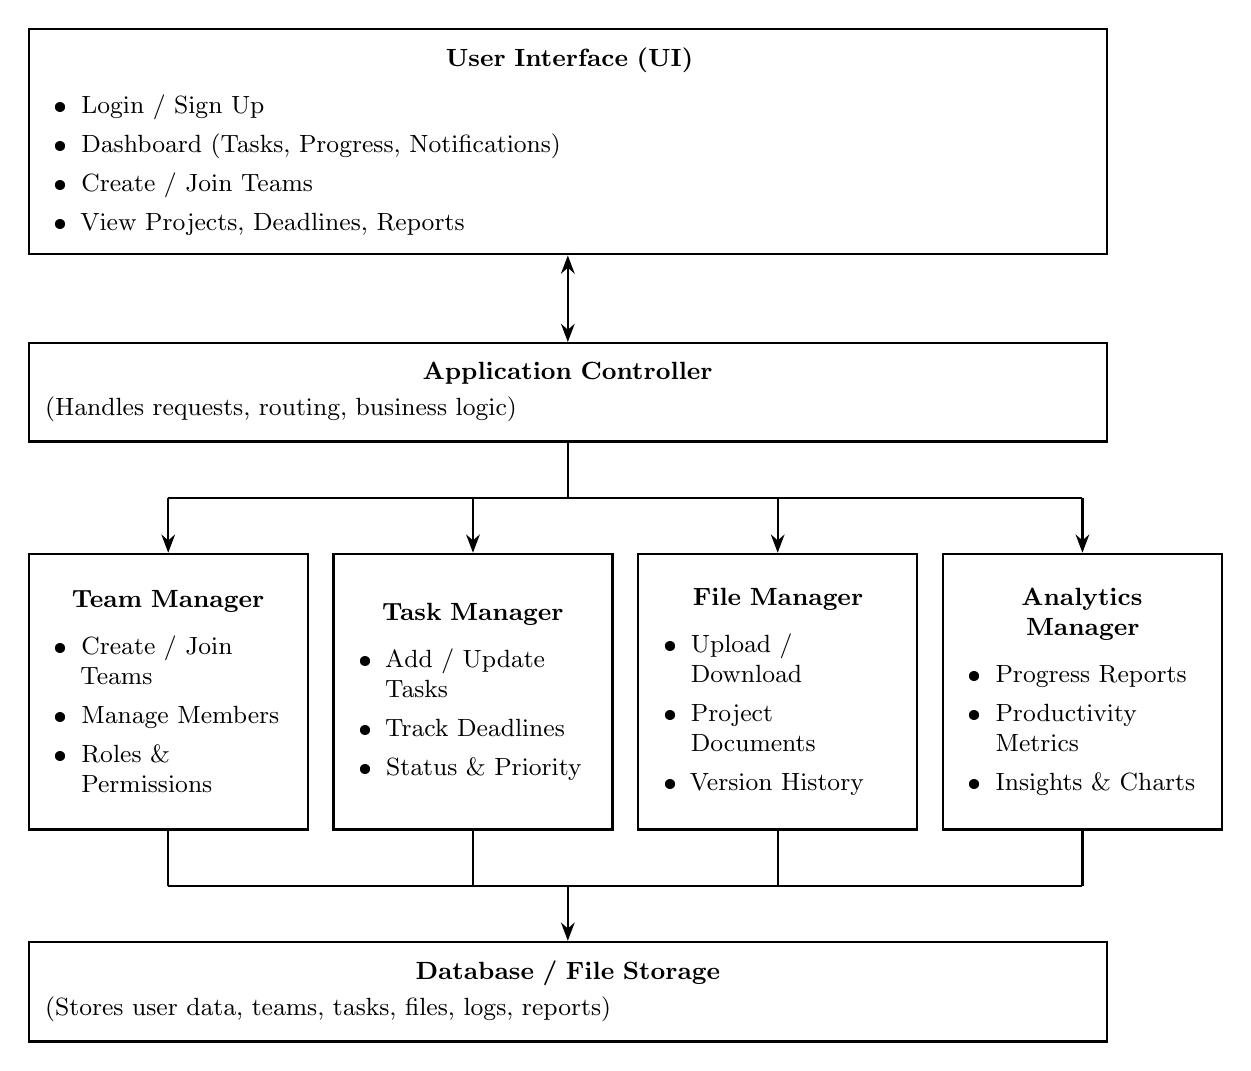
\begin{tikzpicture}[
  >=Stealth, thick,
  boxstyle/.style={draw, align=left, inner sep=7pt, font=\small},
  rowbox/.style={boxstyle, text width=3.05cm, minimum height=3.5cm}
]

\node[boxstyle, text width=13.2cm] (ui) {
\centering\textbf{User Interface (UI)}\par\vspace{3pt}
\raggedright
\begin{itemize}[leftmargin=12pt,itemsep=1pt,topsep=1pt]
\item Login / Sign Up
\item Dashboard (Tasks, Progress, Notifications)
\item Create / Join Teams
\item View Projects, Deadlines, Reports
\end{itemize}};

\node[boxstyle, text width=13.2cm, below=11mm of ui] (ctrl) {
\centering\textbf{Application Controller}\\[2pt]
{(Handles requests, routing, business logic)}};

\node[rowbox, below=14mm of ctrl.south west, anchor=north west] (team) {
\centering\textbf{Team Manager}\par\vspace{3pt}
\raggedright\begin{itemize}[leftmargin=12pt,itemsep=1pt,topsep=1pt]
\item Create / Join Teams
\item Manage Members
\item Roles \& Permissions
\end{itemize}};

\node[rowbox, right=3mm of team] (task) {
\centering\textbf{Task Manager}\par\vspace{3pt}
\raggedright\begin{itemize}[leftmargin=12pt,itemsep=1pt,topsep=1pt]
\item Add / Update Tasks
\item Track Deadlines
\item Status \& Priority
\end{itemize}};

\node[rowbox, right=3mm of task] (file) {
\centering\textbf{File Manager}\par\vspace{3pt}
\raggedright\begin{itemize}[leftmargin=12pt,itemsep=1pt,topsep=1pt]
\item Upload / Download
\item Project Documents
\item Version History
\end{itemize}};

\node[rowbox, right=3mm of file] (analytics) {
\centering\textbf{Analytics Manager}\par\vspace{3pt}
\raggedright\begin{itemize}[leftmargin=12pt,itemsep=1pt,topsep=1pt]
\item Progress Reports
\item Productivity Metrics
\item Insights \& Charts
\end{itemize}};

\node[boxstyle, text width=13.2cm, below=14mm of team.south west, anchor=north west] (db) {
\centering\textbf{Database / File Storage}\\[2pt]
{(Stores user data, teams, tasks, files, logs, reports)}};

\draw[<->] (ctrl.north) -- (ui.south);

\coordinate (midtop) at ($(ctrl.south)!0.5!(team.north)$);
\draw (ctrl.south) -- (ctrl.south |- midtop);
\draw (team.north |- midtop) -- (analytics.north |- midtop);
\draw[->] (team.north |- midtop) -- (team.north);
\draw[->] (task.north |- midtop) -- (task.north);
\draw[->] (file.north |- midtop) -- (file.north);
\draw[->] (analytics.north |- midtop) -- (analytics.north);

\coordinate (midbot) at ($(team.south)!0.5!(db.north)$);
\draw (team.south |- midbot) -- (analytics.south |- midbot);
\draw (team.south) -- (team.south |- midbot);
\draw (task.south) -- (task.south |- midbot);
\draw (file.south) -- (file.south |- midbot);
\draw (analytics.south) -- (analytics.south |- midbot);
\draw[->] (db.north |- midbot) -- (db.north);

\end{tikzpicture}
\end{center}
\end{answerbox}
\clearpage

% PAGE 6
\SubHeading{Project Outcome / Deliverables (1 pts)}
\Instruction{(Describe what are the outcomes / deliverables of the project. Max 200 words).}
\begin{answerbox}
\begin{itemize}[leftmargin=18pt,itemsep=3pt,topsep=2pt]
\item A C++/Qt desktop prototype for creating student skill profiles and project/hackathon requirements.
\item A matching engine that retrieves relevant candidates, ranks them using the defined score, and reports skill coverage and remaining gaps.
\item Team formation and validation features covering team size, duplicate membership, coverage, and skill gaps.
\item Source code, project documentation, DSA/OOP mapping, matching-score description, and selected Algorithm Lab work.
\item Local persistence for profiles, requirements, and formed-team information, followed by a final demonstration of the planned matching flow.
\end{itemize}
\end{answerbox}
\vspace{10pt}
\SubHeading{Assumptions}
\Instruction{(Describe the assumptions (if any) you are making to solve the problem. Max 100 words).}
\begin{answerbox}
\begin{itemize}[leftmargin=18pt,itemsep=3pt,topsep=2pt]
\item Students provide reasonably accurate information about skills, experience, and availability.
\item Project requirements use identifiable skills or roles and include a practical team-size limit.
\item The first version runs locally and uses files instead of external APIs or cloud services.
\item Candidate data is small enough to be handled in memory, and the score is treated as a decision aid rather than a guarantee of team success.
\end{itemize}
\end{answerbox}
\vspace{10pt}
\SubHeading{References}
\Instruction{(Provide a list of resources or references you utilised for the completion of this deliverable. You may provide links).}
\begin{answerbox}
\begin{enumerate}[leftmargin=19pt,itemsep=2pt,topsep=1pt]
\item Thareja, R. \textit{Data Structures Using C}. Oxford University Press.
\item Balagurusamy, E. \textit{Object Oriented Programming with C++}. McGraw Hill Education.
\item Cormen, T. H., Leiserson, C. E., Rivest, R. L., \& Stein, C. \textit{Introduction to Algorithms}. MIT Press.
\item Weiss, M. A. \textit{Data Structures and Algorithm Analysis in C++}. Pearson.
\item Stroustrup, B. \textit{The C++ Programming Language}. 4th ed., Addison-Wesley.
\item Gamma, E., Helm, R., Johnson, R., \& Vlissides, J. \textit{Design Patterns: Elements of Reusable Object-Oriented Software}. Addison-Wesley.
\item The Qt Company. \textit{Qt Documentation}. \url{https://doc.qt.io/qt-6/}
\item cppreference.com. \textit{C++ Language and Standard Library Reference}. \url{https://en.cppreference.com/}
\end{enumerate}\end{answerbox}

\end{document}